% Created 2022-05-31 mar 01:23
% Intended LaTeX compiler: pdflatex
\documentclass[11pt]{article}
\usepackage{xcolor}
\usepackage[utf8]{inputenc}
\usepackage[T1]{fontenc}
\usepackage{graphicx}
\usepackage{longtable}
\usepackage{wrapfig}
\usepackage{rotating}
\usepackage[normalem]{ulem}
\usepackage{amsmath}
\usepackage{amssymb}
\usepackage{capt-of}
\usepackage{hyperref}
\author{Uri Mtz}
\date{\textit{<2022-05-31 mar>}}
\title{Unsubscribeservices}
\hypersetup{
 pdfauthor={Uri Mtz},
 pdftitle={Unsubscribeservices},
 pdfkeywords={},
 pdfsubject={},
 pdfcreator={Emacs 28.1 (Org mode 9.6)}, 
 pdflang={English},
 colorlinks=false,
 linkbordercolor=blue,
 pdfborderstyle={/S/U/W 1}}\begin{document}

\maketitle
\tableofcontents

\section{Anzuelo}
\label{sec:orge280d21}
\begin{center}
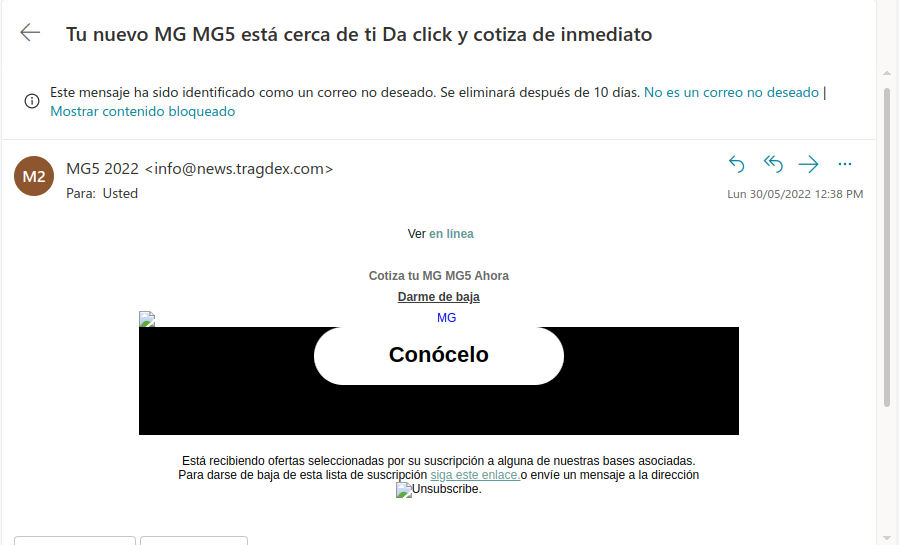
\includegraphics[width=.9\linewidth]{./assets/20220531-001335.png}
\end{center}
\section{Información remitente y título}
\label{sec:org3c87779}
El remitente, identificado por Outlook como \emph{MG5 2022}, bajo el correo \uline{info@news.tragdex.com} envía un correo titulado \textbf{Tu nuevo MG MG5 está cerca de ti Da click y cotiza de inmediato}

\url{https://tragdex.com} es el dominio del correo remitente, si se entra a su página, lleva a una página estática que muestra un texto en inglés, mencionando que sólo son una página que \emph{envía mails a sus usuarios registrados}, más adelante muestra una forma que invita al usuario a registrarse, esta forma acepta cualquier dato sin verificar si tiene un sentido alguna información, únicamente el nombre y apellido deben contener más de 3 caracteres y el correo debe tener un dominio válido, si se registra un correo cualquiera, inmediatamente no llega ningún tipo de correo de confirmación.

Al pie de la forma contiene una nota que menciona algunas supuestas empresas que patrocina este dominio, estas páginas y empresas parecen ser reales, sin embargo se necesita más investigación.

\begin{center}
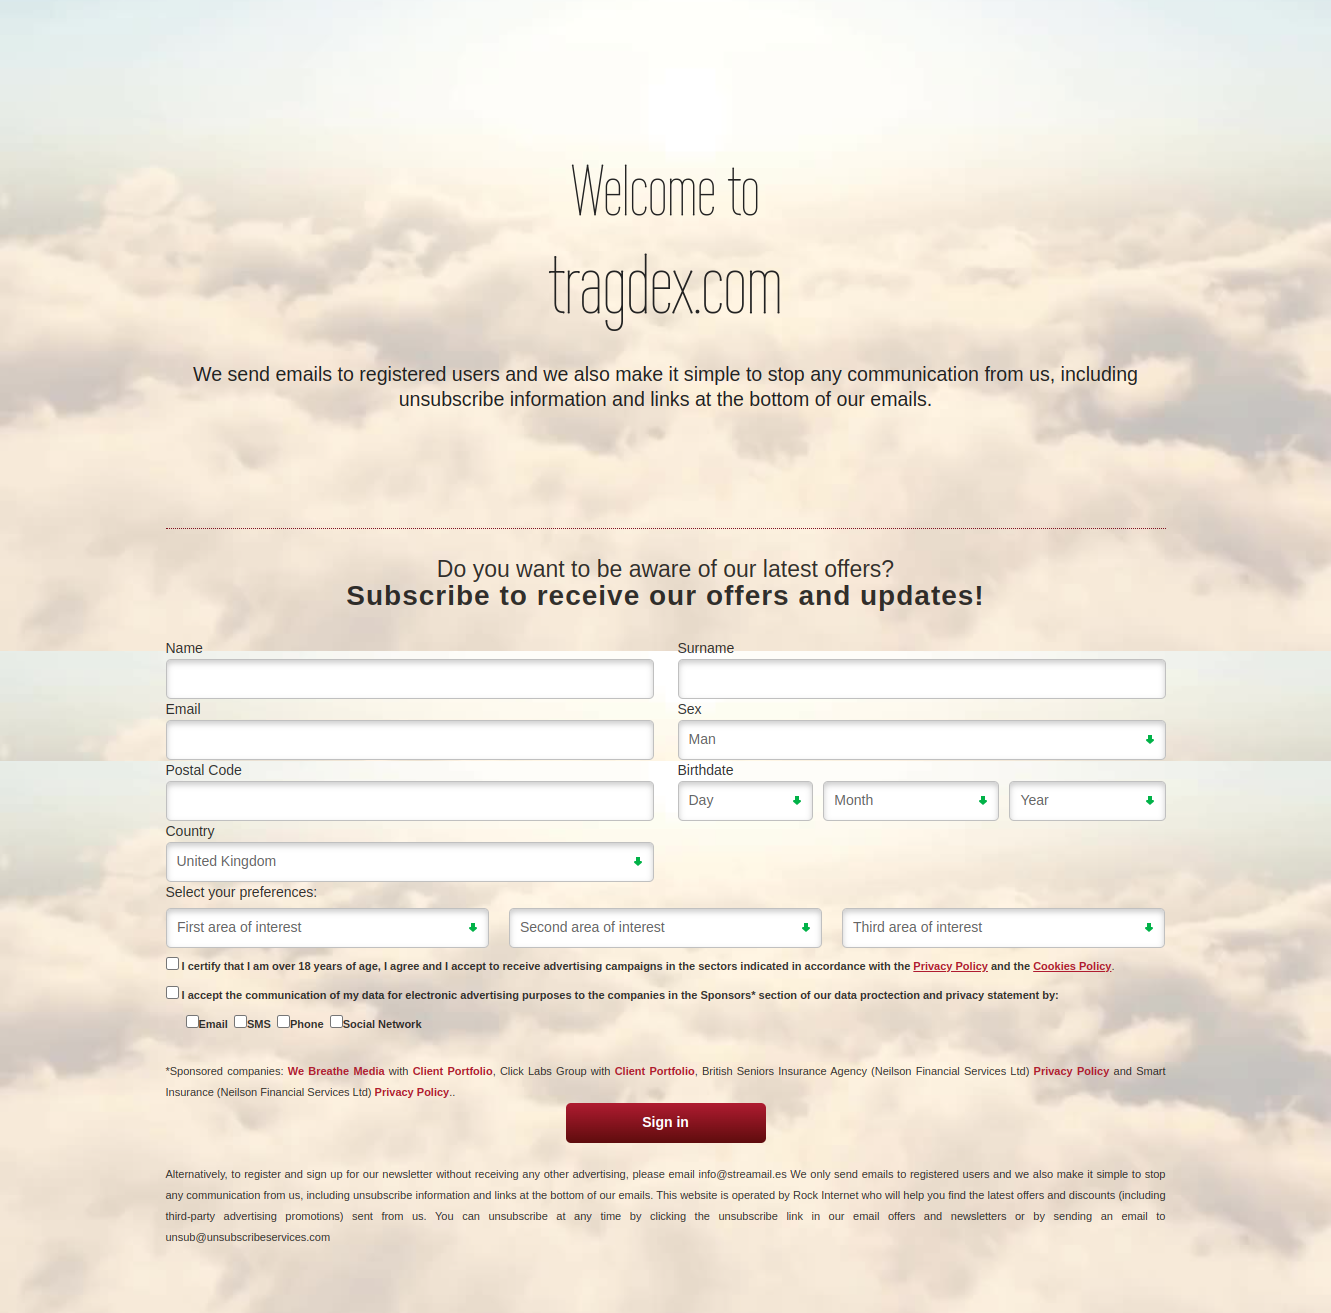
\includegraphics[width=.9\linewidth]{./assets/screencapture-tragdex-2022-05-31-00_52_15.png}
\end{center}

Este dominio fue registrado con ``Don Dominio'', una web europea (española al parecer), que te permite comprar dominios.
\section{Contenido}
\label{sec:orge9a7939}
El correo en si mismo no es peligroso, ya que no contiene ningún archivo adjunto, sin embargo intenta mostrarse como un anuncio acerca de una cotización.

Los elementos nombrados:
\begin{itemize}
\item \emph{en línea}
\item \emph{darme de baja}
\item \emph{MG}
\item \emph{Conócelo}
\item \emph{siga este enlace}
\end{itemize}

Contienen un enlace que lleva a la dirección:

\url{https://mailing.monskuar.com/}

\subsection{Contenido del enlace}
\label{sec:orgdb24fc2}
El enlace lleva a una página que solicita dar clic en un botón para comprobar que no eres un robot, este botón está hecho con un elemento \texttt{div} dentro del código html, el cual no ejecuta ningún script malicioso, sin embargo la página posee un código que funciona como redireccionamiento en cuanto el usuario hace clic en el botón, el script es el siguiente:

\texttt{var divR=document["\textbackslash{}x67\textbackslash{}x65\textbackslash{}x74\textbackslash{}x45\textbackslash{}x6C\textbackslash{}x65\textbackslash{}x6D\textbackslash{}x65\textbackslash{}x6E\textbackslash{}x74\textbackslash{}x42\textbackslash{}x79\textbackslash{}x49\textbackslash{}x64"]("\textbackslash{}x63\textbackslash{}x72\textbackslash{}x31");document["\textbackslash{}x67\textbackslash{}x65\textbackslash{}x74\textbackslash{}x45\textbackslash{}x6C\textbackslash{}x65\textbackslash{}x6D\textbackslash{}x65\textbackslash{}x6E\textbackslash{}x74\textbackslash{}x42\textbackslash{}x79\textbackslash{}x49\textbackslash{}x64"]("\textbackslash{}x63\textbackslash{}x72\textbackslash{}x31")["\textbackslash{}x61\textbackslash{}x64\textbackslash{}x64\textbackslash{}x45\textbackslash{}x76\textbackslash{}x65\textbackslash{}x6E\textbackslash{}x74\textbackslash{}x4C\textbackslash{}x69\textbackslash{}x73\textbackslash{}x74\textbackslash{}x65\textbackslash{}x6E\textbackslash{}x65\textbackslash{}x72"]("\textbackslash{}x63\textbackslash{}x6C\textbackslash{}x69\textbackslash{}x63\textbackslash{}x6B",redir);function redir()\{var b\_url;var url;b\_url= document["\textbackslash{}x67\textbackslash{}x65\textbackslash{}x74\textbackslash{}x45\textbackslash{}x6C\textbackslash{}x65\textbackslash{}x6D\textbackslash{}x65\textbackslash{}x6E\textbackslash{}x74\textbackslash{}x42\textbackslash{}x79\textbackslash{}x49\textbackslash{}x64"]("\textbackslash{}x63\textbackslash{}x72\textbackslash{}x31")["\textbackslash{}x67\textbackslash{}x65\textbackslash{}x74\textbackslash{}x41\textbackslash{}x74\textbackslash{}x74\textbackslash{}x72\textbackslash{}x69\textbackslash{}x62\textbackslash{}x75\textbackslash{}x74\textbackslash{}x65"]('\textbackslash{}x64\textbackslash{}x61\textbackslash{}x74\textbackslash{}x61\textbackslash{}x2D\textbackslash{}x63\textbackslash{}x72\textbackslash{}x31');url= atob(b\_url);window["\textbackslash{}x6C\textbackslash{}x6F\textbackslash{}x63\textbackslash{}x61\textbackslash{}x74\textbackslash{}x69\textbackslash{}x6F\textbackslash{}x6E"]["\textbackslash{}x72\textbackslash{}x65\textbackslash{}x70\textbackslash{}x6C\textbackslash{}x61\textbackslash{}x63\textbackslash{}x65"](url)\}}

El dominio \url{https://monskuar.com}, es un dominio registrado con ``Don Dominio'', la página es una página estática similar a la que es dominio del correo remitente, a diferencia de la primera, esta se muestra en español, sin embargo esto es debido a la detección del país, las características son similares, sin embargo esta página no te permite registrarte debido a que no está configurado de manera correcta su captcha.

\begin{center}
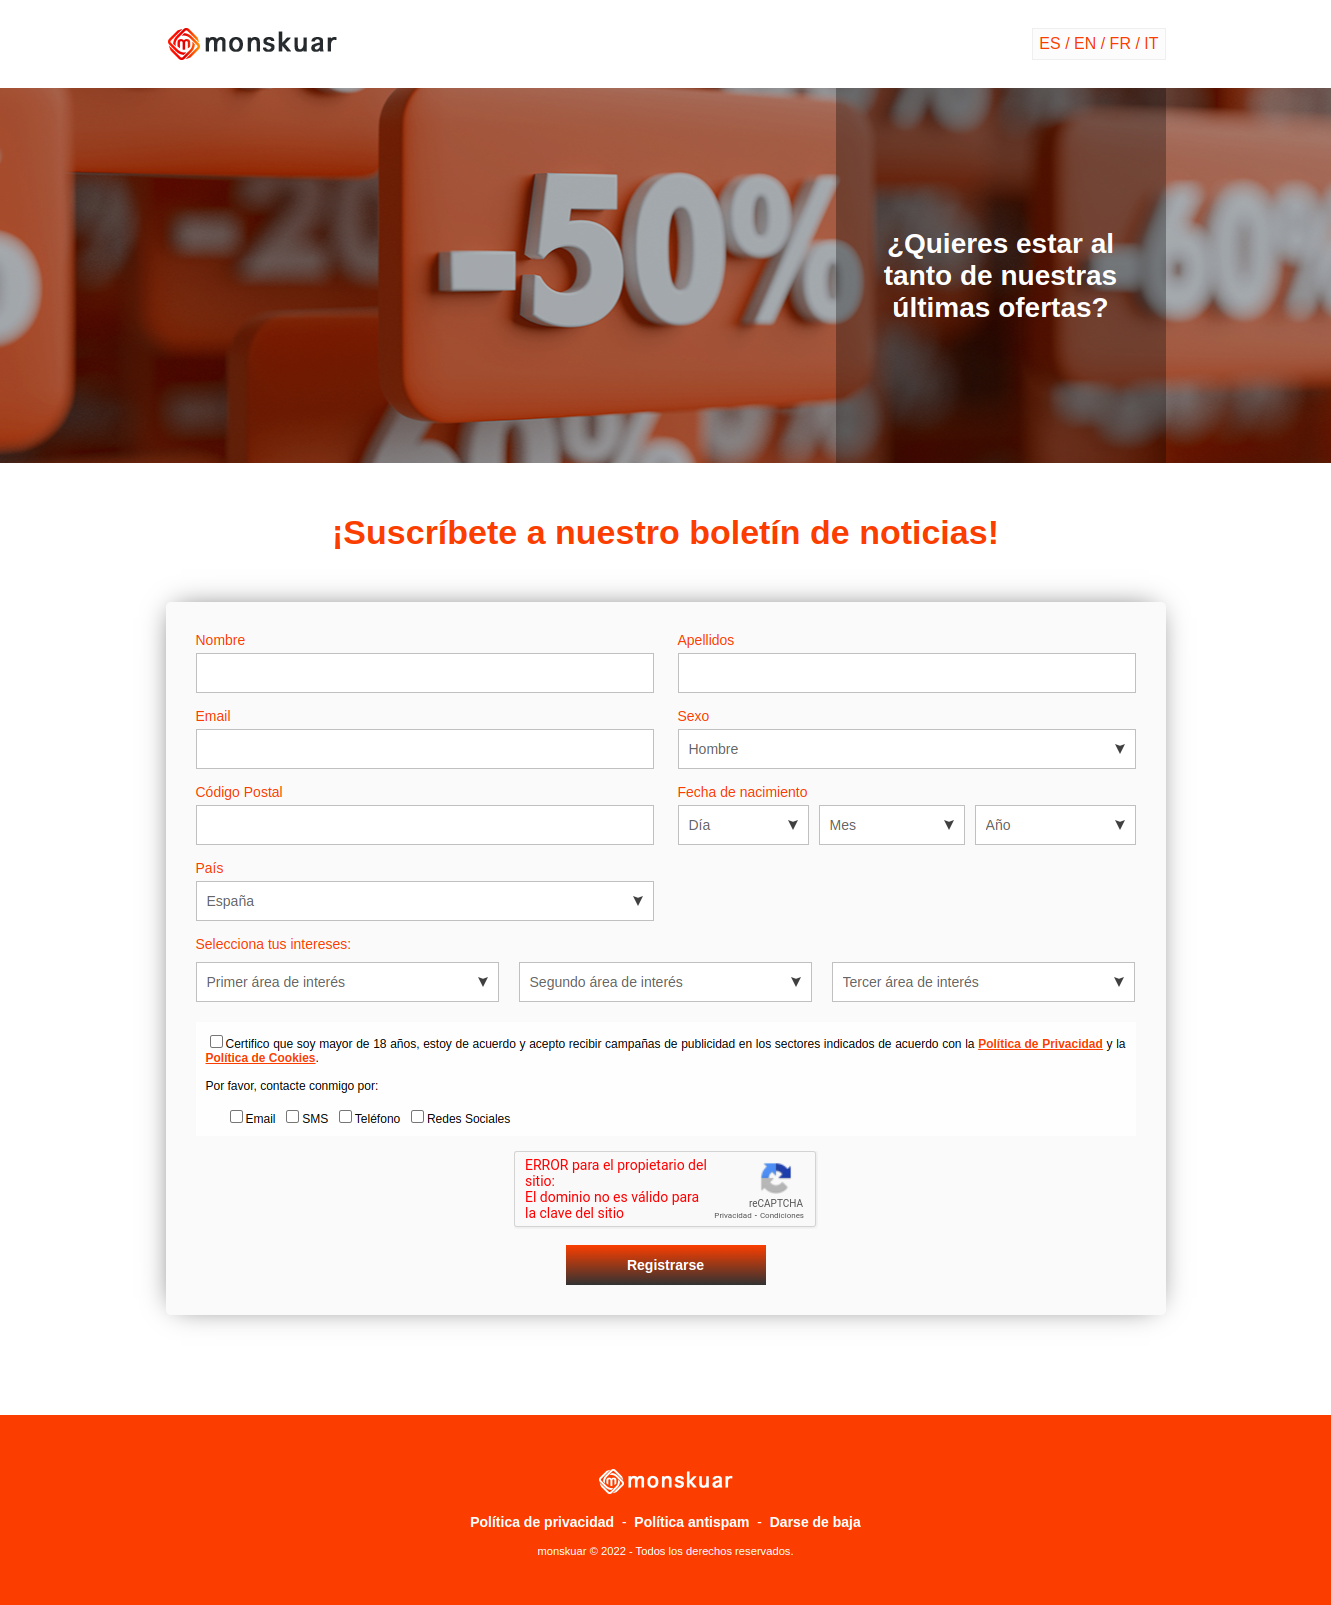
\includegraphics[width=.9\linewidth]{./assets/screencapture-monskuar-2022-05-31-00_59_54.png}
\end{center}

Al finalizar el redireccionamiento desde \url{https://monskuar.com}, lleva hacia \url{https://unsubscribeservices.com}, página que supuestamente te permite eliminar tu supuesta suscripción a su lista de suscripción. Promete que la solicitud será procesada en las próximas 48 horas.

Por tratarse de un redireccionamiento, los enlaces acarrean el correo, por lo que será mostrado automáticamente en la forma, únicamente solicita comprobar que no eres un robot usando un captcha.

\begin{center}
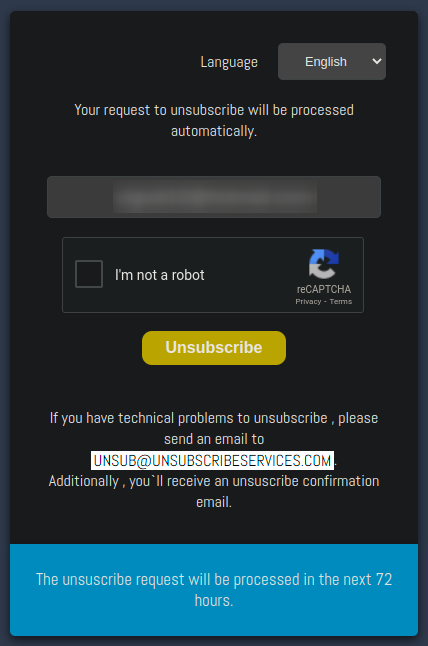
\includegraphics[width=.9\linewidth]{./assets/20220531-010337.png}
\end{center}

La búsqueda de información acerca del dominio únicamente muestra que fue registrado con ``OVH'', mientras el resto de la información se mantiene privada.

Una breve búsqueda en internet muestra \url{https://www.mywot.com/scorecard/unsubscribeservices.com} como uno de los primeros resultados, el cual muestra 3 reseñas, las cuales describen que el sitio únicamente es usado para suscribirte a una lista de correo de spam y que la supuesta desuscripción nunca sucede.

Este dominio y todo lo que conllevó anteriormente está ligado a algún usuario o empresa española, por lo tanto, gran parte de sus objetivos son de habla hispana.
\subsection{Tomando medidas de seguridad}
\label{sec:org5f81627}
Para evitar caer en este tipo de estafas se recomienda lo siguiente:
\begin{itemize}
\item Estos correos entran normalmente a la carpeta de \emph{correo no deseado} o \emph{spam}, por lo que pueden ser ignorados sin ningún riesgo.
\item Si el correo llega a la bandeja principal, la manera de identificar esta estafa es el sentido común, en este caso, si no ordenaste una cotización del producto mencionado, es muy probable que sea una estafa.
\item Si cualquiera de los enlaces llevan al mismo destino a pesar de que sea contradictorio, por ejemplo, \emph{conócelo} y \emph{darme de baja} son frases contradictorias, sin embargo ambas llevan a la misma dirección, por lo tanto es altamente probable que se trate de una estafa.
\item Bloquear al remitente usando su cliente de correo o su proveedor, Gmail provee funciones de filtro para que automáticamente se eliminen o rechacen los correos de ese remitente
\item Tomando medidas de seguridad
Para evitar caer en este tipo de estafas se recomienda lo siguiente:
\begin{itemize}
\item Estos correos entran normalmente a la carpeta de \emph{correo no deseado} o \emph{spam}, por lo que pueden ser ignorados sin ningún riesgo.
\item Si el correo llega a la bandeja principal, la manera de identificar esta estafa es el sentido común, en este caso, si no ordenaste una cotización del producto mencionado, es muy probable que sea una estafa.
\item Si cualquiera de los enlaces llevan al mismo destino a pesar de que sea contradictorio, por ejemplo, \emph{conócelo} y \emph{darme de baja} son frases contradictorias, sin embargo ambas llevan a la misma dirección, por lo tanto es altamente probable que se trate de una estafa.
\item Bloquear al remitente usando su cliente de correo o su proveedor, Gmail provee funciones de filtro para que automáticamente se eliminen o rechacen los correos de ese remitente.
\end{itemize}
\end{itemize}
\end{document}
